\section{Theoretical Analysis} \label{section:theo}


\par In this section, a theoretical analysis of the circuit was conducted. In the introduction, we can see analysed circuit.

First of all we got to keep in mind that that our circuit is divided in two different stages. The first one corresponds to the gain stage with a NPN transistor and the second is the output stage with a PNP transistor. The components and their functions of each stage has already been described in the Simulation Analysis as well as the goal of each stage.

In order to analyse a stage we need to study both Operating point and incremental analysis.
First, we shut down the AC independent sources and  and compute a simple analysis of the circuit. This way we obtain $Z_i$ and $Z_o$. Moreover, to compute the DC response we can say the capacitors behave like open circuits because there is only DC.

To analyse the incremental response we have to create a model of the transistor (and the rest of the gain stage) similar to Fig.2. Studying the circuit we get $v_{o1}=-g_m * (r_o||R_c) * v_{\pi}$ and $v_{\pi}= \frac{R_B||r_{\pi}}{R_B||r_{\pi}+R_s} * v_s $ which lead us to $A_{v1} = \frac{v_{o1}}{v_s} = -g_m * (r_o||R_c)*\frac{R_B||r_{\pi}}{R_B||r_{\pi}+R_s}$


\begin{figure}[h] \centering
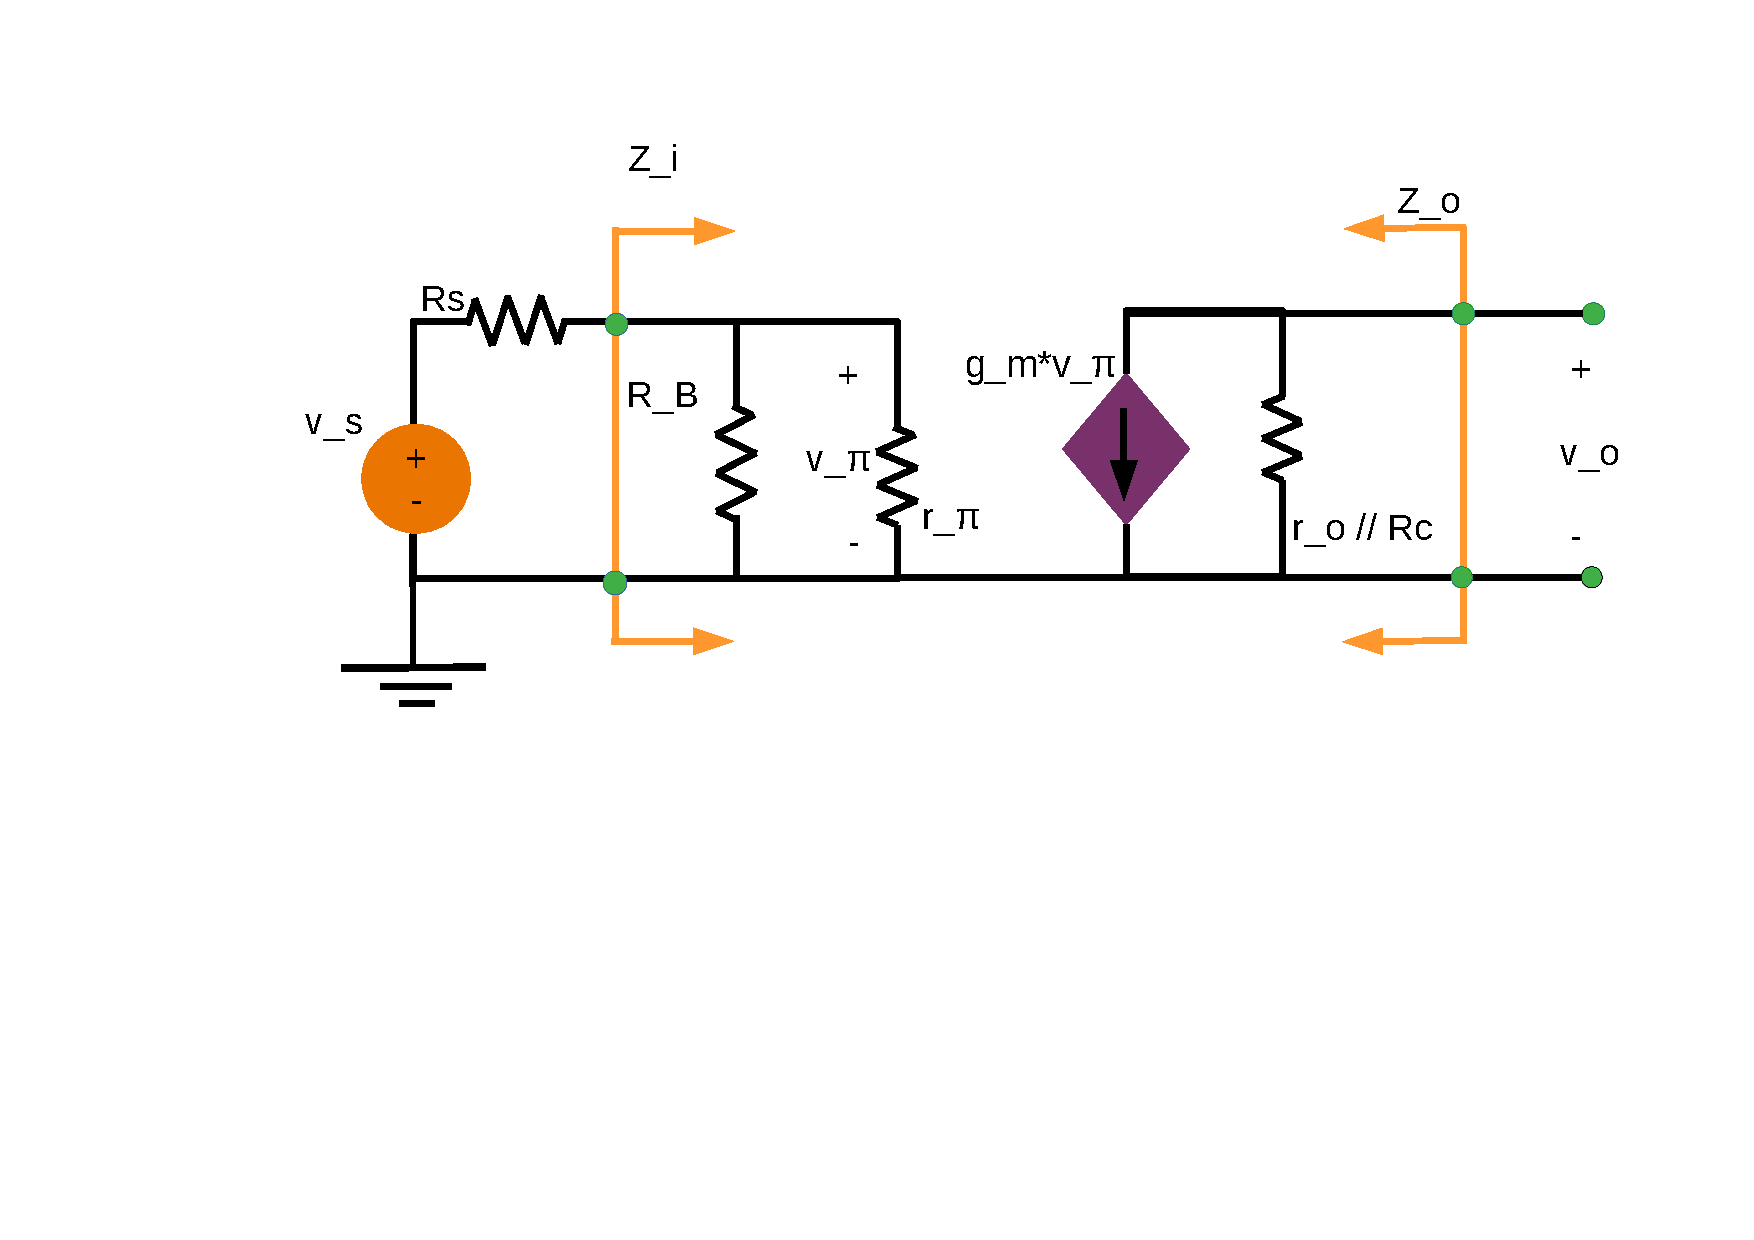
\includegraphics[width=0.65\linewidth]{Incremental_Gain.pdf}
\caption{Model for the gain stage incremental analysis}
\label{sdf}
\end{figure}

For the DC response of the output stage, we follow the same logic of the gain stage and we easily get $Z_o$. On the other hand, to get the incremental response we have to create another model like Fig.3. Using nodal analysis we end up with $A{v2} = \frac{v_{o1}}{v_i} = \frac{g_{\pi} + g_m }{g_{\pi}+g_z+g_o+g_m}$ for the gain.



\begin{figure}[h] \centering
\includegraphics[width=0.65\linewidth]{Incremental_Output.pdf}
\caption{Model for the output stage incremental analysis}
\label{s}
\end{figure}



Finally, we calculated $i_o$ to then compute $Z_o=\frac{v_{o}}{i_o}$ using the provided equations. The gain is given by $A_V = A_{V1}*{AV2}$
All the important results obtained are shown in the table and in the figure bellow. 


\begin{figure}[h] \centering
\includegraphics[width=0.65\linewidth]{A.eps}
\caption{Voltage Gain of the circuit}
\label{sh}
\end{figure}


\begin{table}[ht]
  \centering
  \begin{tabular}{|l|r|}
    \hline    
    {\bf Name} & {\bf Value} \\ \hline
    \input{../mat/ponto2_tab}
  \end{tabular}
  \caption{Impedences and Gains of both stages an the full circuit.}
  \label{tab:p2}
\end{table}


















